% For plaintext use only
\documentclass{article}

\usepackage{xltxtra}
\usepackage{amsmath}
\usepackage{amssymb}
\usepackage{tikz}
\usepackage{unicode-math}
\usepackage{fontspec}
\usepackage{faktor}
\setmathfont{xits-math.otf}

\tikzset{node distance=2cm, auto}

\author{Víctor López Juan}
\title{Chapter 4}

\begin{document}

\begin{enumerate}
  \item[4.]
    % Every monoid in the category of groups is an internal group.

    % Internal group:

    % In the same way that groups in the category of groups are abelian
    % internal groups, we will have that monoids in the category of groups
    % are internal groups.

    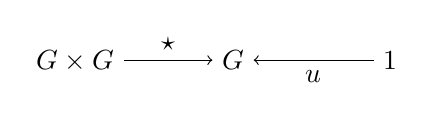
\begin{tikzpicture}
      \node  (GG)  {$G \times G$};
      \node  (G) [right of=GG] {$G$};
      \node  (T) [right of=G] {$1$};
      
      \draw[->] (GG) to node {$\star$} (G);
      \draw[->] (T) to node {$u$} (G);
    \end{tikzpicture}

    Observe that $u$ is the inclusion of the trivial group in $G$.

    Now:

    \begin{itemize}
      \item The underlying set of the monoid is $G$. The operation is $m$.
      \item $m$ is associative, because $m$ is part of a monoid in the
        category.

      \item $m$ respects identity, again because it's a monoid.

      \item $m$ is a group homomorphism.

        $m(g₁·h₁, g₂·h₂) = m((g₁,g₂)·(h₁,h₂)) = m(g₁,g₂)·m(h₁,h₂)$
                                              

        Therefore, the operation $m$ is the same as the original operation
        in the group, and is therefore, an inverse. Also, only commutative
        groups can form a monoid in Group.
    \end{itemize}
        

  \item[8.]

    \begin{itemize}
      \item It is a congruence:

        % f ~ g implies dom,cod(f) = dom,cod(g) %
        % f ~ g implies bfa ~ bga

        \item By definition, the domain and the codomain match.
        \item
          Let f, g such that $f ~ g$.
          

          \begin{itemize}
            \item $~$ is an equivalence relation. This is derived from the
              fact that equality is an equivalence relation, and the double
              implication.

               $$dom,cod(bfa) = \langle dom(a), cod(b) \rangle = dom,cod(bga)$$

            \item
              
              Let $H : D → E$ such that $HF = HG$. Then $H(f) = H(g)$

              H(bfa) = H(b)H(f)H(a) = H(b)H(g)H(a) = H(bga)
              
          \end{itemize}

        \item

          % D/~ is the coequalizer of F and G

          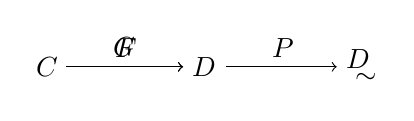
\begin{tikzpicture}
            \node (C) {$C$};
            \node (D) [right of=C] {$D$};
            \node (DQ) [right of=D] {$\faktor{D}{\sim}$};

            \draw[->] (C) to node {$F$} (D);
            \draw[->] (C) to node {$G$} (D);
            \draw[->] (D) to node {$P$} (DQ);
          \end{tikzpicture}

          \begin{itemize}
            \item % PF = PG

              P(F(C)) = P(G(C)), because F(C) = G(C)


                dom,cod(Fα) = dom,cod(Gα)

                If HF = HG, then H(Fα) = H(Gα).

              Therefore: F(α) ~ G(α)

              Therefore: PF(α) = PG(α)

              Now, if there is a functor $Z : D -> X$, such that
              $ZF = ZG$, then there is a unique functor $\bar{Z} : \faktor{D}{\sim} → X$, such that

              $\bar{Z} \circ P = Z$. 

              $\bar{Z} = Z \circ I$, where $I$ is a choice function
              from $\faktor{D}{\sim}$ to the original set.

              \begin{itemize}
                \item
                    For every $x$, let $\bar{x} = I(P(x))$
                    
                    \begin{equation*}
                    \bar{Z} P(x) = Z (I P(x)) =          % projection
                                 = Z (I P(\bar{x}) )) =  % x ~ \bar{x}
                                 = Z (\bar{x})           % \bar{x} is the representative
                                 = Z (x)                 % x ~ \bar{x}
                    \end{equation*}  
                    
                \item
                    Uniqueness:
                    
                    Let $\bar{Z}^\prime : \faktor{D}{\sim} → X$ such
                    that $\bar{Z}^\prime \circ P = Z$.

                    
                    Then $\bar{Z}^\prime(x) = \bar{Z}^\prime(P(I(x))) =
                                          = Z(I(x)) = \bar{Z}(x)$.
             \end{itemize}
        \end{itemize}
    \end{itemize}    
\end{enumerate}

\end{document}
  
